%%%%%%%%%%%%%%%%%%%%%%%%%%%%%%%%%%%%%%%%%%%%%%%%%%%%%%%%%%
\begin{frame}
  \begin{center}
    {\Large Introduction to TensorFlow Data}
	
	{\tiny (Ref: Building a High-Performance Data Pipeline with Tensorflow 2.x - Mayank Kumar )}
  \end{center}
\end{frame}

%%%%%%%%%%%%%%%%%%%%%%%%%%%%%%%%%%%%%%%%%%%%%%%%%%%%%%%%%%%
\begin{frame}[fragile]\frametitle{Data Pipeline}
\begin{itemize}
\item Goal:  Having an efficient, scalable as well as generic pipeline 
\item Multiple sources, multiple formats (image, text, csv, server log file, videos, audio files, etc.)
\item Tensorflow  tf.data module can be easily customized to consume these data efficiently and send it to the model for further computations. 
\end{itemize}
\end{frame}

%%%%%%%%%%%%%%%%%%%%%%%%%%%%%%%%%%%%%%%%%%%%%%%%%%%%%%%%%%%
\begin{frame}[fragile]\frametitle{Tensorflow Data}
\begin{itemize}
\item  \lstinline|tf.data| module
\item \lstinline|tf.data.Dataset| abstraction that represents a sequence of elements, in which each element consists of one or more components, which can be used as a source to consume data.
\item E.g. a single element in spam classifier dataset has two components: a text data and its label 
\item \lstinline|tf.data.Dataset| behaves as a python iterator, which can be easily accessed using a python $for$ loop.
\end{itemize}
\end{frame}

%%%%%%%%%%%%%%%%%%%%%%%%%%%%%%%%%%%%%%%%%%%%%%%%%%%%%%%%%%
\begin{frame}
  \begin{center}
    {\Large CSV in TensorFlow Data}
	
	{\tiny (Ref: Building a High-Performance Data Pipeline with Tensorflow 2.x - Mayank Kumar )}
  \end{center}
\end{frame}

%%%%%%%%%%%%%%%%%%%%%%%%%%%%%%%%%%%%%%%%%%%%%%%%%%%%%%%%%%%
\begin{frame}[fragile]\frametitle{From Small CSV}
\lstinline|tf.data.Dataset.from_tensor_slices|

\begin{itemize}
\item CSV small enough to fit in memory.
\item Read it into Pandas dataframe
\item \lstinline|tf.data.Dataset.from_tensor_slices| to convert dataframe object to \lstinline|tf.data.Dataset|
\end{itemize}

\begin{lstlisting}
df = pd.read_csv("sample.csv")
dataset = tf.data.Dataset.from_tensor_slices(dict(df))
\end{lstlisting}
\end{frame}

%%%%%%%%%%%%%%%%%%%%%%%%%%%%%%%%%%%%%%%%%%%%%%%%%%%%%%%%%%%
\begin{frame}[fragile]\frametitle{From Python Generator}
\lstinline|tf.data.Dataset.from_generator|

\begin{itemize}
\item Uses python generators for consuming the dataset.
\item Can incorporate transformation logic on python side.
\item Transformation happens on-the-go during data consumption.
\end{itemize}

\begin{lstlisting}
def read_csv(filepath,skip_rows):
	with open(filepath,'r') as csvfile:
		data = csv.reader(csvfile, delimiter=",")
		for index, row in enumerate(data):
			if index < skip_rows:
				continue
			yield row[0],row[1],row[2]
			
dataset = tf.data.Dataset.from_generator(read_csv, output_types =(tf.string,
																					tf.int8,tf.float16)
\end{lstlisting}
\end{frame}

%%%%%%%%%%%%%%%%%%%%%%%%%%%%%%%%%%%%%%%%%%%%%%%%%%%%%%%%%%%
\begin{frame}[fragile]\frametitle{From CSV}
\lstinline|tf.data.experimental.make_csv_dataset|

\begin{itemize}
\item Batch-wise loading
\item Shuffling possible
\end{itemize}

\begin{lstlisting}
path = tf.keras.utils.get_file(filepath)
dataset = tf.data.Dataset.make_csv_dataset(path,batch_size=32,
																						label_name = target_column,
																						select_columns=feature-columns,
																						shuffle=True)
\end{lstlisting}
\end{frame}

%%%%%%%%%%%%%%%%%%%%%%%%%%%%%%%%%%%%%%%%%%%%%%%%%%%%%%%%%%%
\begin{frame}[fragile]\frametitle{From BIG Data}
\lstinline|tf.data.TFRecordDataset|

\begin{itemize}
\item Used to consume any amount of data in a most efficient way.
\item To build a streaming input pipeline that can stream over the content of one or more TFRecord files.
\item Store any dataset like CSVs, Images, Texts, etc., into a set of TFRecord files, using \lstinline|TFRecordWriter|
\item For training, need to get original format back using \lstinline|tf.train.Example| in case of scalar features and \lstinline|tf.serialize_tensor| in case of non-scalar features
\end{itemize}

\begin{center}
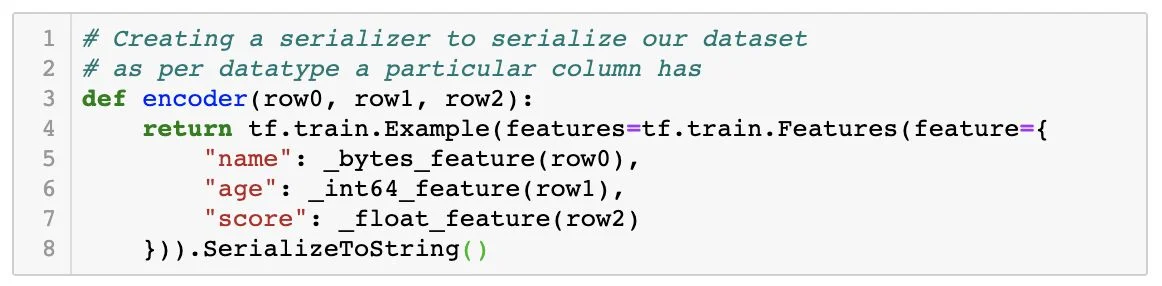
\includegraphics[width=\linewidth,keepaspectratio]{tfdata1}
\end{center}
\end{frame}

%%%%%%%%%%%%%%%%%%%%%%%%%%%%%%%%%%%%%%%%%%%%%%%%%%%%%%%%%%%
\begin{frame}[fragile]\frametitle{From BIG Data}
\lstinline|tf.data.TFRecordDataset|

\begin{center}
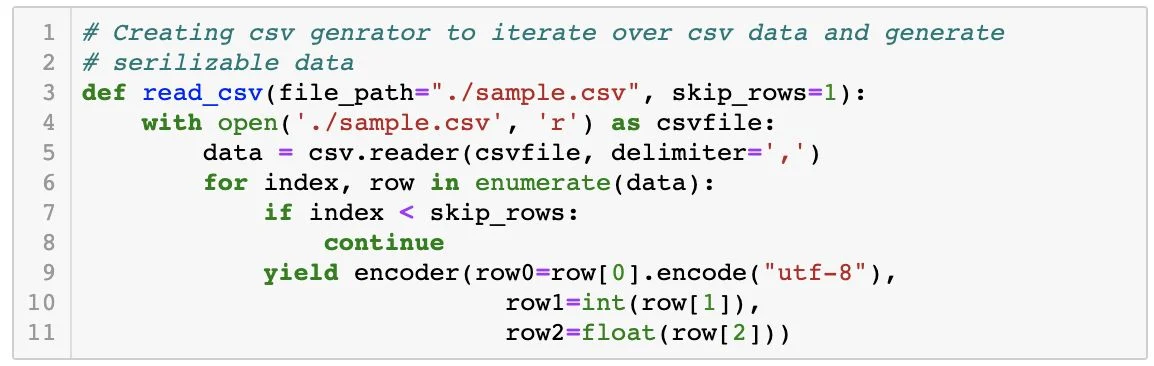
\includegraphics[width=\linewidth,keepaspectratio]{tfdata2}

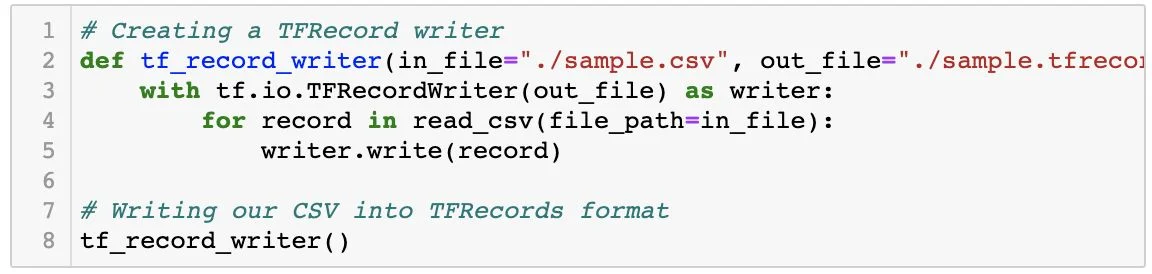
\includegraphics[width=\linewidth,keepaspectratio]{tfdata3}


\end{center}
\end{frame}

%%%%%%%%%%%%%%%%%%%%%%%%%%%%%%%%%%%%%%%%%%%%%%%%%%%%%%%%%%%
\begin{frame}[fragile]\frametitle{From BIG Data}
\lstinline|tf.data.TFRecordDataset|

\begin{center}

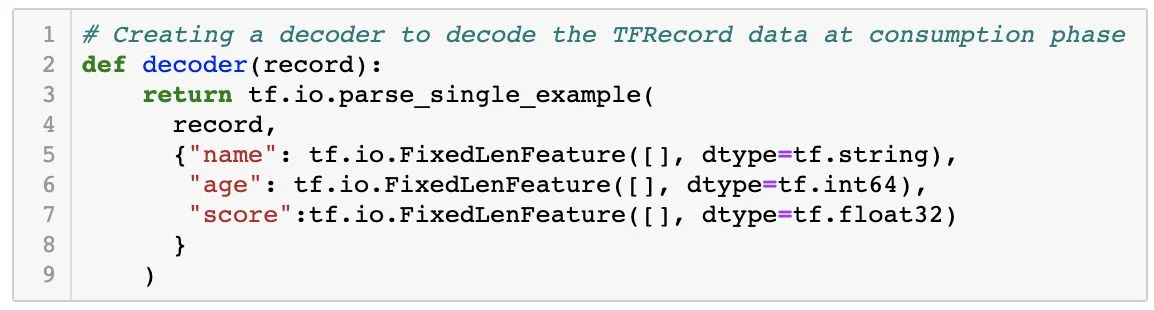
\includegraphics[width=\linewidth,keepaspectratio]{tfdata4}

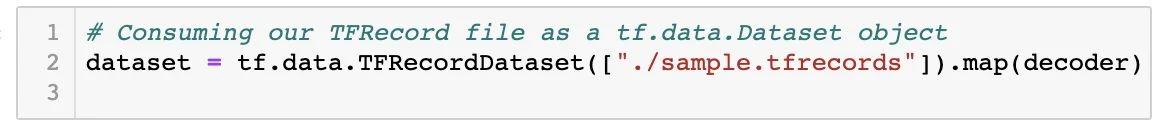
\includegraphics[width=\linewidth,keepaspectratio]{tfdata5}


\end{center}
\end{frame}

%%%%%%%%%%%%%%%%%%%%%%%%%%%%%%%%%%%%%%%%%%%%%%%%%%%%%%%%%%%
\begin{frame}[fragile]\frametitle{After Dataset}
\begin{itemize}
\item Use \lstinline|.prefetch()| to send next batch data to GPUs or TPUs while current batch is getting completed
\item Use \lstinline|.interleave()| with parallelism for transformation of the dataset, if transformation is needed at the time of consumption phase. 
\item Use \lstinline|.cache()| to cache some computations like transformation which may be overlapping during each epoch.
\end{itemize}
\end{frame}
